\section{Hauptteil}

\subsection{Web Services}
\begin{frame}{Web Services}
    \ldots
\end{frame}

\subsection{Dokumentbeschreibungssprachen}
\begin{frame}{XSD}
    \ldots
\end{frame}

\begin{frame}{WADL}
    \ldots
\end{frame}

\subsection{Codegenerierung}
\begin{frame}{Codegenerierung}

    \begin{block}{Vorteile}
        \begin{itemize}
            \item Produktivitässteigerung
            \item hohe Konsistenz des Generats
            \item zentrale Stelle für Änderungen (Eingabemodell)
        \end{itemize}
    \end{block}
\end{frame}

\begin{frame}{}
    \begin{figure}
        \resizebox{\textwidth}{!}{
            \begin{tikzpicture}[
        node distance=12mm and 8mm,
        every node/.style={font=\scriptsize}
    ]
    % Blocks
    \node(abstractDescription)[greyBlock]{Abstrakte\\Beschreibung\\der Spreadshirt-API};
    \node(dummy1)[dummy, right=of abstractDescription]{};
    \node(wadlAnalysis)[greyBlock, above=of abstractDescription]{Analyse\\WADL-Datei};
    \node(restModel)[greyBlock, right=of wadlAnalysis]{REST-\\Modell};
    \node(xsdAnalysis)[greyBlock, below=of abstractDescription]{Analyse\\XSD-Datei};
    \node(schemaModel)[greyBlock, right=of xsdAnalysis]{Schema-\\Modell};
    \node(modelCombine)[greyBlock, right=of dummy1]{Kombinierer};
    \node(applicationModel)[greyBlock, right=of modelCombine]{Applikations-\\Modell};
    \node(generator)[greyBlock, right=of applicationModel]{Generator};
    \node(languageModel)[greyBlock, right=of generator]{Zielsprachen-\\Modell};
    \node(languageFactory)[greyBlock, below=of generator]{Language-\\Factory};
    \node(filePrinter)[greyBlock, right=of languageModel]{Ausgabemodul\\(File Printer)};
    \node(languageVisitor)[greyBlock, above=of filePrinter]{Language-\\Visitor};
    \node(library)[greyBlock, double copy shadow, right=of filePrinter]{Bibliotheks-\\Dateien};
    \node(staticFiles)[greyBlock, double copy shadow, below=of library]{Statische Dateien};

    %\node(languagemodel)[greyBlock, right= of generator]{Sprachenmodell\\\emph{Abstrakter Syntaxbaum}};
    % Lines  
    \path[arrow, ->] (abstractDescription) -- (wadlAnalysis);
    \path[arrow, ->] (abstractDescription) -- (xsdAnalysis);
    \path[arrow, ->] (wadlAnalysis) -- (restModel);
    \path[arrow, ->] (xsdAnalysis) -- (schemaModel);
    \path[arrow, ->] (restModel) -- (modelCombine);
    \path[arrow, ->] (schemaModel) -- (modelCombine);
    \path[arrow, ->] (modelCombine) -- (applicationModel);
    \path[arrow, ->] (applicationModel) -- (generator);
    \path[arrow, ->] (languageFactory) -- (generator);
    \path[arrow, ->] (generator) -- (languageModel);
    \path[arrow, ->] (languageModel) -- (filePrinter);
    \path[arrow, ->] (languageVisitor) -- (filePrinter);
    \path[arrow, ->] (filePrinter) -- (library);
    \path[arrow, ->] (staticFiles) -- (library);

    %\path[arrow, ->] (infrastructurecode) -- (generator);
\end{tikzpicture}

        }
        \caption{Sequenzdiagramm des Generators}
    \end{figure}
\end{frame}

\subsection{Datenmodelle \& Codegenerator}
\begin{frame}{Datenmodelle \& Codegenerator}
    \begin{figure}
        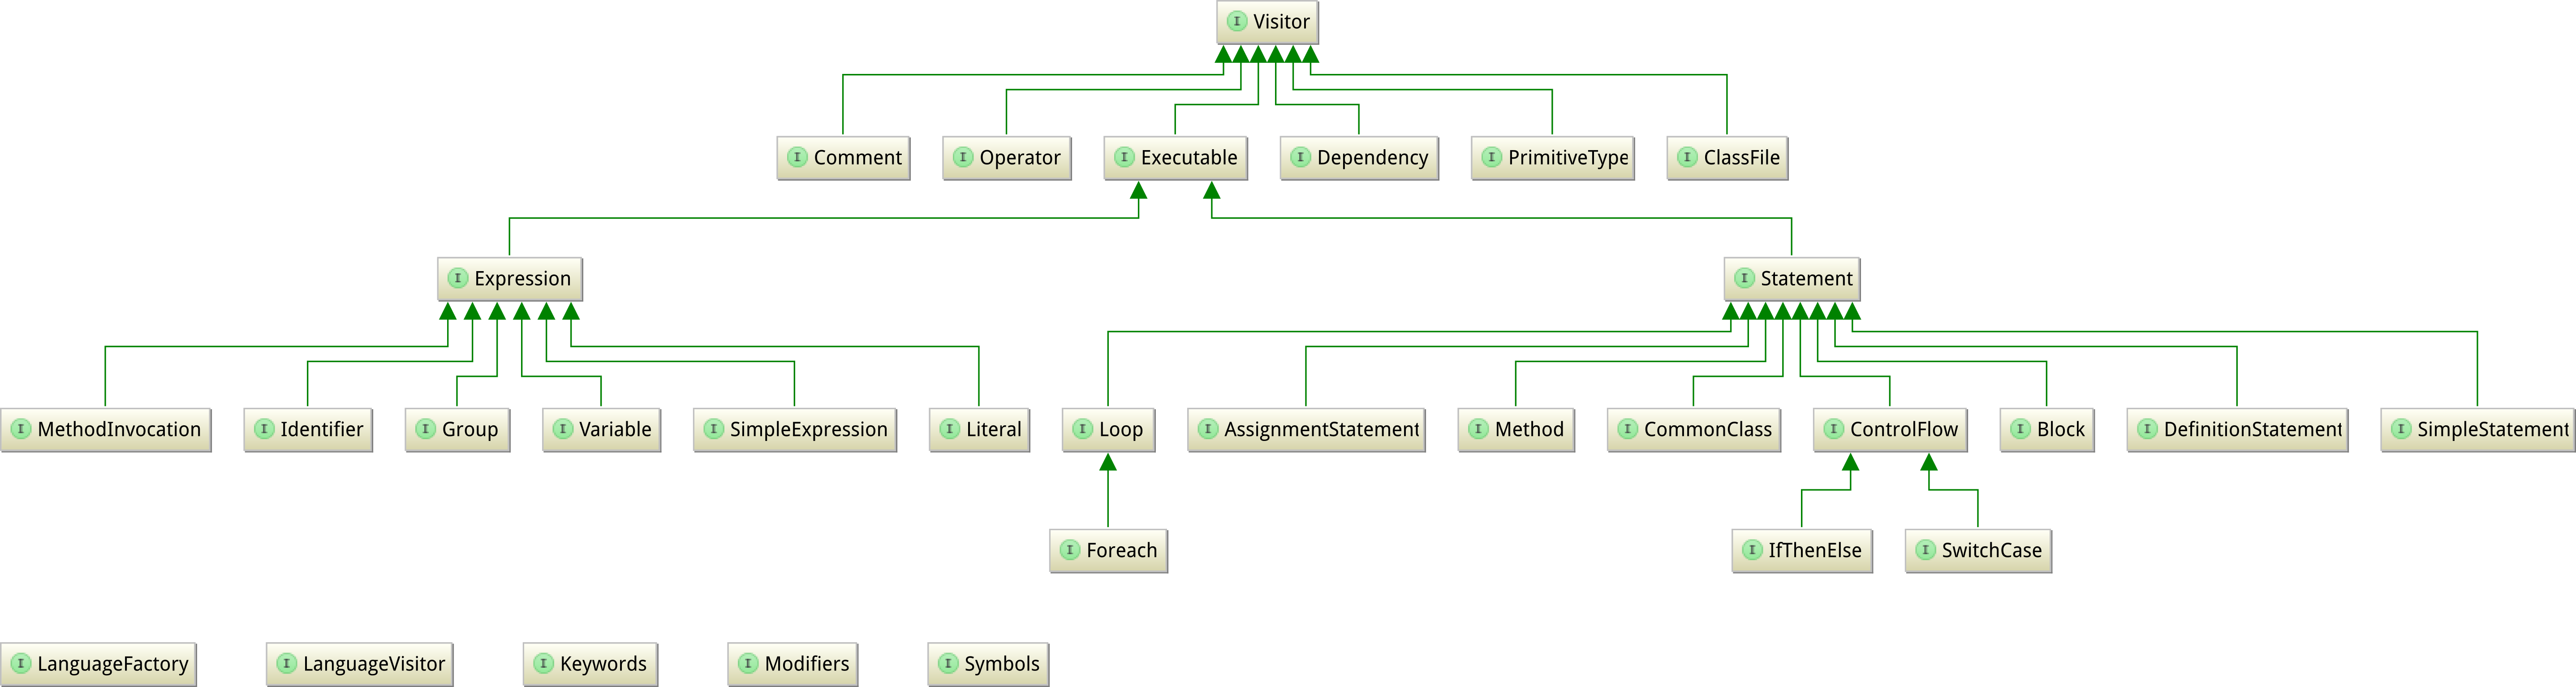
\includegraphics[width=\textwidth]{resources/languagemodel}
    \end{figure}
\end{frame}

\subsection{Client-Bibliothek}
\begin{frame}{Client-Bibliothek}
    \ldots
\end{frame}
